\documentclass[a4paper,12pt]{article}
\author{Adam Ilyas 725819}
\title{
CS-E5740 Complex Networks, \\
Answers to exercise set 3
}

\usepackage{amsfonts}
\usepackage{verbatim}
\usepackage{amsmath}
\usepackage{amsfonts}
\usepackage{graphicx}
\usepackage[english]{babel}
\usepackage{listings}

\begin{document}
\vspace{8pt}

\maketitle

Acknowledgements: Lukas Haug, Bianca Lachennmann, Christoph Berger, Zeyneb Erdogan
\section{Implementing the Barabási-Albert (BA) model}

The Barabási-Albert scale-free network model is a model of network growth, where new nodes
continuously enter the network and make links to existing nodes with a probability that is
linearly proportional to their degree. The steps required for generating a Barabási-Albert scale-
free network with N nodes are as follows:

\begin{itemize}
\item Create a small seed network which has at least m nodes, where m is the number of links a
  new node creates to already existing nodes. \textit{For the purpose of this exercise, use 3-clique as the seed network.}
\item Add new nodes to the network until your network has $N$ nodes, such that each entering node has $m$ links and connects to existing nodes proportional to their degrees.
\item[a) ]
  \begin{itemize}
    \item[--] \textbf{Implement} a Python function for generating Barabási-Albert networks. Then generate a network with $N = 200$ and $m = 1$ (a tree!).
    \item[--] \textit{Write} down degree of the node with the highest degree in your generated network.
    \item[--] \textit{Write} down total number of links in your generated network.
    \item[--] \textbf{visualize} it with networkx using the spring layout i.e. \texttt{nx.draw\_spring(G)}. You should be able to spot some nodes that have many connections, while most of the
nodes have few connections.
\end{itemize}

\begin{figure}
  \centering
  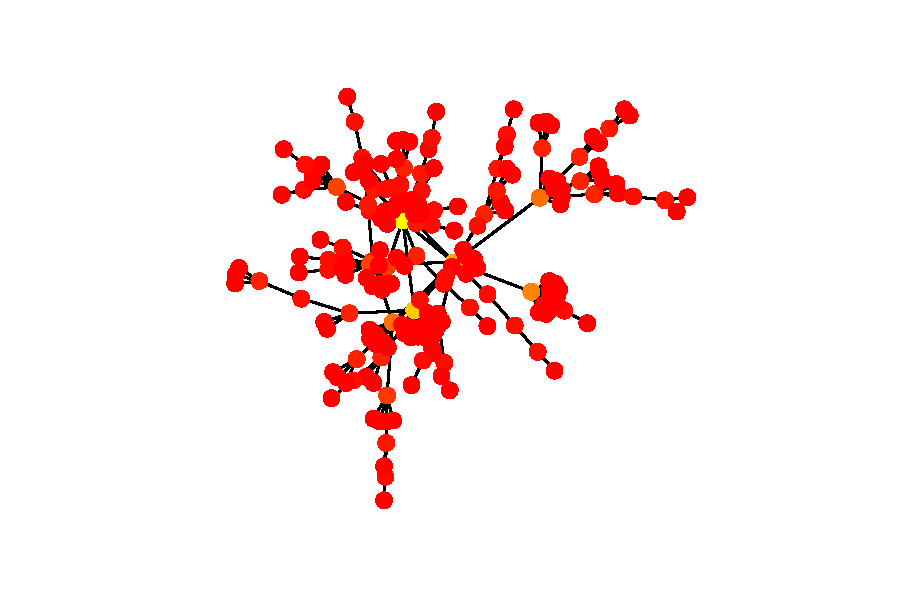
\includegraphics[width=0.75\textwidth]{assets/BA_visualized.pdf}
    \caption{BA network with $N = 200, m = 1$}
\end{figure}


\item[b) ]

\begin{itemize}
\item[--] \textbf{Generate} a new network using parameters $N = 10^4$ with $m = 2$ and plot the logarithmically binned probability density function for degree, $P(k)$ (on double logarithmic axes, \texttt{ax.loglog}).
\item[--] \textbf{Compare} your result with the theoretical prediction of $P(k) = 2m (m + 1) / [k (k + 1) (k + 2)]$ (shown in the next exercise).
\item[--] \textbf{Plot} both the experimental and theoretical distributions on the same axes.
\end{itemize}

\begin{minipage}{\textwidth}
  \centering
  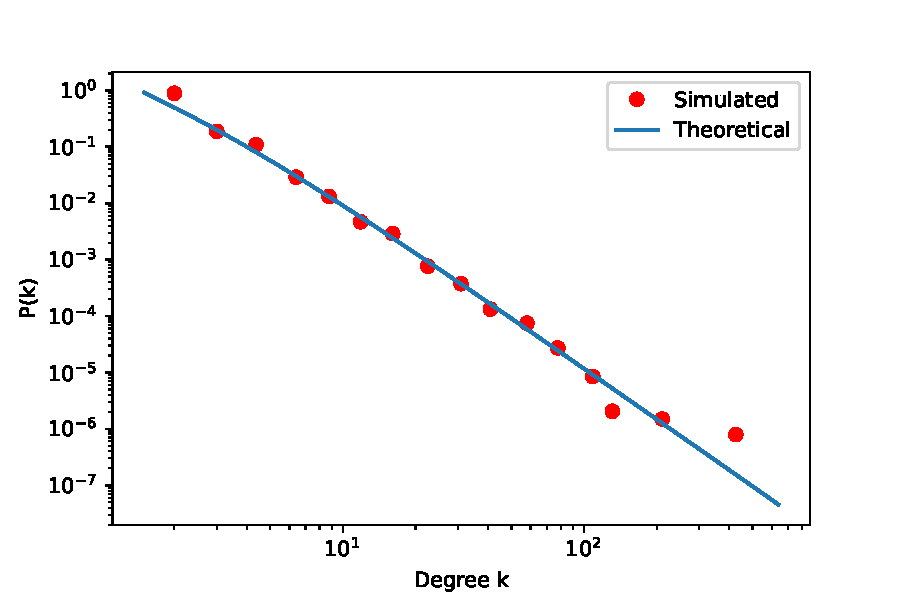
\includegraphics[width=0.75\textwidth]{assets/BA_degree_distribution.pdf}
\end{minipage}

\end{itemize}

\section{Deriving the degree distribution for the BA-model $P (k) = \frac{2m (m + 1)}{[k (k + 1) (k + 2)]}$}

Write an equation for the changes
in the fraction of vertices of degree $k$, $p_k$, as function of time and find stationary solutions. In such solutions, $p_k$ does not change anymore when the network grows,
corresponding to an infinite network size.
This stationary solution for $p_k$ when $N \rightarrow \infty$ equals the degree distribution
$P(k)$ of the network.

\begin{itemize}
\item[a) ] Let $p_{k,N}$ be the density of vertices of degree $k$ in a network that, at time $t$,
  has altogether $N(t)$ vertices. Thus, $n_{k,N}$  is the number of vertices of degree k in
the network:
$$n_{k,N} = N(t) p_{k,N}$$

At each time step, one vertex is added, and hence $N(t) = t + N_0$ , where
$t \in Z$ denotes the time step of the network growth process.

Since $N_0$ is small, we can
approximate $N \approx ≈ t$. In the following, $N$ will be used for $N(t)$ for readability.
In the BA model, the probability $\Pi_i$ that a new edge attaches to a particular vertex of
degree $k_i$ equals:
\begin{equation} \Pi_i = \frac{k_i}{\sum_{j=1}^N k_j} \end{equation}

The sum of degree of $N \approx t$ vertices is $\sum_{j=1}^N k_j = 2m \times t$ where $m$ is the number of new edges attached to a new node.

\textbf{We can derive}, the probability $\prod(k)$ that a new edge attaches
to any vertex of degree $k$ in a network of $N$ vertices:
\begin{equation}
  \begin{split}
    \Pi (k) & = n_{k,N} \times \Pi_i\\
    & = n_{k,N} \times \frac{k}{\sum_{j=1}^N k_j}\\
    & = n_{k,N} \times \frac{k}{2mt} \\
    & = N(t) p_{k,N} \times \frac{k}{2mt} = \frac{t p_{k,N}k}{2mt}\\
    & =  \frac{k p_{k,N}}{2m}\\ 
  \end{split}
\end{equation}

\item[b) ] Changes of the average numbers of vertices of degree $k$.
  From Eq. (2), the average number$^2$ of vertices of degree $k$ that gain
  an edge when a single new vertex with m edges is added is
  $$m \times kp_{k,N}/2m = \frac{1}{2} kp_{k,N}$$

This means that the number $n_{k,N}$ of vertices with degree k must decrease by this amount,
since these vertices become vertices of degree $k + 1$. Let’s mark this as:

\begin{equation}
n_k^- = \frac{1}{2}kp_{k,N}
\end{equation}

But at the same time, there is an increase $n^+_k$ as well. For vertices with degree $k > m$
this is equal to the average number of vertices that used to have degree $k - 1$ and became
vertices of degree k by gaining an edge. For vertices with $k = m$, $n^+_k = 1$.
\textbf{Explain why?}

\textbf{Because the vertices with degree k = m will be the new nodes with m edges. (We assume that after a long time, the other nodes will have multiple new nodes attached to them as the network grows)} 

Net change of the number of vertices of degree k as the network grows
in size from N to N + 1:  

\begin{equation}
  \begin{split}
    n^+_k - n^-_k  & = (N+1)p_{k,N+1} - Np_{k,N}\\ 
    & = 
    \begin{cases}
  \frac{1}{2}(k-1)p_{k-1,N} - \frac{1}{2}kp_{k,N}  & k > m\\    
   1 - \frac{1}{2}kp_{k,N} & otherwise    
\end{cases}
\end{split}
\end{equation}

\clearpage

\item[c) ] Now, let the network grow towards the infinite network size limit and consider
stationary solutions of the two equations you just wrote. In this case, there are no longer
changes in the probability density $p_k$ , and so you can write
\begin{itemize}
\item[] $p_{k,N+1} = p_{k,N} = p_k$
\item[] $p_{k-1,N} = p_{k-1}$
\item[] $p_{m,N +1} = p_{m,N} = p_m$
\end{itemize}

\textbf{Write down equations} for $p_k$ and $p_m$ . The density $p_k$ should now be of the
form $F(k) \times p_{k-1}$ , where $F(k)$ is some prefactor depending on $k$ alone. $p_m$ should be a function of $m$ only, $p_m = G(m)$.

\begin{minipage}{0.5\linewidth}
\centering
\begin{equation*}
  \begin{split}
    p_k & = (N+1)p_{k} - Np_{k}\\
    & = (N+1)p_{k,N+1} - Np_{k,N}\\
    & = \frac{1}{2}(k-1)p_{k-1,N} - \frac{1}{2}kp_{k,N}\\
    & = \frac{1}{2}(k-1)p_{k-1} - \frac{1}{2}kp_{k}\\
    \\
    p_k & = \frac{k-1}{k+2}p_{k-1}
  \end{split}
  \end{equation*}
\end{minipage}\hfill
\begin{minipage}{0.5\linewidth}
\centering
\begin{equation*}
  \begin{split}
    p_m & = 1 - \frac{1}{2}kp_{k,N}, \quad m =k\\
    & = 1 - \frac{1}{2}mp_{m,N}\\
    & = 1 - \frac{1}{2}mp_{m}\\
    \\
    p_m & = \frac{2}{2+m}
  \end{split}
  \end{equation*}
\end{minipage}


\item[d) ] Now things get recursive: $p_k$ depends on $p_{k−1}$ . At the same
time, we have a formula for $p_m$ which depends only on $m$, which is the smallest degree in
our network. Your final task is to derive a formula for $p_k$ , so that $p_k$ is a function of $k$ and $m$ only.

\end{itemize}

\end{document}